% DMA Session 2: SQL für Datenexploration
% 180-Minuten-Block (Vorlesung + Übung interwoven)

\documentclass[usenames,dvipsnames,10pt,aspectratio=169]{beamer}
\usepackage[T1]{fontenc}
\usepackage[utf8]{inputenc}
\usepackage{verbatim}

% Theme loaded via symlinks (update beamerTemplate/ for CD changes)
\usetheme{ims}

\usepackage{booktabs}
\usepackage{multicol}
\usepackage{listings}
\usepackage{xcolor}
\usepackage{graphicx}
\usepackage{tikz}
\usetikzlibrary{shapes.geometric, arrows.meta, positioning, calc, fit, backgrounds}
\usepackage{pifont}

% ===== CLICKABLE AGENDA WITH PROGRESS INDICATOR =====
\usepackage{hyperref}
\hypersetup{colorlinks=false, pdfborder={0 0 0}}

% Phase counter for progress tracking
\newcounter{currentphase}
\setcounter{currentphase}{0}

% TikZ styles for diagrams
\tikzset{
    sqlbox/.style={rectangle, rounded corners, minimum width=2.5cm, minimum height=0.8cm,
        text centered, draw=IMSBlue, fill=IMSBlue!15, font=\ttfamily\small},
    sqlarrow/.style={-{Stealth[length=2.5mm]}, thick, IMSOrange},
    nullbox/.style={rectangle, rounded corners, minimum width=1.8cm, minimum height=0.6cm,
        text centered, draw=gray, fill=gray!20, font=\small},
}

% SQL Listing Style
\lstdefinestyle{sql}{
    language=SQL,
    basicstyle=\ttfamily\footnotesize,
    keywordstyle=\color{IMSBlue}\bfseries,
    stringstyle=\color{IMSOrange},
    commentstyle=\color{gray}\itshape,
    showstringspaces=false,
    breaklines=true,
    frame=single,
    backgroundcolor=\color{gray!10},
    morekeywords={SERIAL, BOOLEAN, TEXT, COALESCE, IFNULL, NULLIF, ISNULL},
    literate={ü}{{\"u}}1 {ä}{{\"a}}1 {ö}{{\"o}}1 {Ü}{{\"U}}1 {Ä}{{\"A}}1 {Ö}{{\"O}}1 {ß}{{\ss}}1
}

\lstset{style=sql}

% Clickable agenda item
\newcommand{\agendaitem}[3]{%
    \ifnum#1=#2
        \textcolor{IMSOrange}{$\blacktriangleright$ \textbf{\hyperlink{phase#2}{#3}}}%
    \else
        \textcolor{gray!70}{\phantom{$\blacktriangleright$} \hyperlink{phase#2}{#3}}%
    \fi\\[0.3em]%
}

% Progress dots for footline (clickable)
\newcommand{\progressdots}{%
    
\begin{tikzpicture}[baseline=-0.5ex]
        \foreach \i in {1,...,5} {
            \ifnum\value{currentphase}=\i
                \node[circle, fill=IMSOrange, minimum size=0.24cm, inner sep=0pt] at (\i*0.4,0) {\hyperlink{phase\i}{\phantom{oo}}};
            \else
                \ifnum\value{currentphase}>\i
                    \node[circle, fill=IMSBlue!60, minimum size=0.2cm, inner sep=0pt] at (\i*0.4,0) {\hyperlink{phase\i}{\phantom{oo}}};
                \else
                    \node[circle, draw=gray!50, minimum size=0.2cm, inner sep=0pt] at (\i*0.4,0) {\hyperlink{phase\i}{\phantom{oo}}};
                \fi
            \fi
        }
    \end{tikzpicture}%
}

% Add progress indicator to footline
\setbeamertemplate{footline}{%
    \leavevmode%
    \hbox{%
        \begin{beamercolorbox}[wd=.33\paperwidth,ht=2.5ex,dp=1ex,left]{author in head/foot}%
            \usebeamerfont{author in head/foot}\hspace*{2ex}\insertshortauthor
        \end{beamercolorbox}%
        \begin{beamercolorbox}[wd=.34\paperwidth,ht=2.5ex,dp=1ex,center]{title in head/foot}%
            \progressdots
        \end{beamercolorbox}%
        \begin{beamercolorbox}[wd=.33\paperwidth,ht=2.5ex,dp=1ex,right]{date in head/foot}%
            \usebeamerfont{date in head/foot}\insertframenumber{} / \inserttotalframenumber\hspace*{2ex}
        \end{beamercolorbox}%
    }%
    \vskip0pt%
}

% Agenda reminder frame - argument is the current phase number
\newcommand{\showagenda}[1]{%
\setcounter{currentphase}{#1}%
\hypertarget{phase#1}{}%
\begin{frame}{Agenda}
\vfill
\begin{center}
\begin{minipage}{0.55\textwidth}
\large
\agendaitem{#1}{1}{1 ~ Rückblick \& ORDER BY}
\agendaitem{#1}{2}{2 ~ DISTINCT \& LIKE}
\agendaitem{#1}{3}{3 ~ NULL-Werte verstehen}
\agendaitem{#1}{4}{4 ~ Visualisierung: Streudiagramme}
\agendaitem{#1}{5}{5 ~ Zusammenfassung}
\end{minipage}
\end{center}
\vfill
\end{frame}
}

%%%%%%%%%%%%%%%%%%%%%%%%%%%%%%%%%%%%%%%%%%%%%%%%%%%%%%%%%%%%%%%%%%%%%%%%%%%%%%%%%%%%%
\title[DMA 02]{Datenmanagement \& -analyse}
\subtitle{Vorlesung 2: SQL für Datenexploration}
\date{Sommersemester 2026}
\author{Prof. Dr. Christoph M. Flath}
\institute{Data Driven Decisions Group, Universität Würzburg}
%%%%%%%%%%%%%%%%%%%%%%%%%%%%%%%%%%%%%%%%%%%%%%%%%%%%%%%%%%%%%%%%%%%%%%%%%%%%%%%%%%%%%

\begin{document}

\begin{frame}
\titlepage
\end{frame}

%%%%%%%%%%%%%%%%%%%%%%%%%%%%%%%%%%%%%%%%%%%%%%%%%%%%%%%%%%%%%%%%%%%%%%%%%%%%%%%%%%%%%
\section*{Agenda}
%%%%%%%%%%%%%%%%%%%%%%%%%%%%%%%%%%%%%%%%%%%%%%%%%%%%%%%%%%%%%%%%%%%%%%%%%%%%%%%%%%%%%

\begin{frame}{Agenda}
\vfill
\begin{center}
\begin{minipage}{0.55\textwidth}
\large
1 ~ Rückblick \& ORDER BY\\[0.3em]
2 ~ DISTINCT \& LIKE\\[0.3em]
3 ~ NULL-Werte verstehen\\[0.3em]
4 ~ Visualisierung: Streudiagramme\\[0.3em]
5 ~ Zusammenfassung\\[0.3em]
\end{minipage}
\end{center}
\vfill
\begin{alertblock}{Lernziele}
Daten sortieren, Duplikate entfernen, Muster finden, mit fehlenden Werten umgehen.
\end{alertblock}
\end{frame}

%%%%%%%%%%%%%%%%%%%%%%%%%%%%%%%%%%%%%%%%%%%%%%%%%%%%%%%%%%%%%%%%%%%%%%%%%%%%%%%%%%%%%
\section{Phase 1: Rückblick \& ORDER BY}
%%%%%%%%%%%%%%%%%%%%%%%%%%%%%%%%%%%%%%%%%%%%%%%%%%%%%%%%%%%%%%%%%%%%%%%%%%%%%%%%%%%%%

\showagenda{1}

\begin{frame}{Rückblick: Was wir schon können}

\begin{tikzpicture}[node distance=0.5cm]
    \node[sqlbox] (select) {SELECT};
    \node[sqlbox, right=of select] (from) {FROM};
    \node[sqlbox, right=of from] (where) {WHERE};
    \node[sqlbox, right=of where, fill=IMSOrange!20, draw=IMSOrange] (result) {Ergebnis};
    \draw[sqlarrow] (select) -- (from);
    \draw[sqlarrow] (from) -- (where);
    \draw[sqlarrow] (where) -- (result);
    \node[below=0.1cm of select, font=\tiny\color{gray}] {Was?};
    \node[below=0.1cm of from, font=\tiny\color{gray}] {Woher?};
    \node[below=0.1cm of where, font=\tiny\color{gray}] {Welche?};
\end{tikzpicture}

\vspace{0.5cm}

\begin{itemize}
    \item \texttt{SELECT} -- Spalten auswählen
    \item \texttt{WHERE} -- Zeilen filtern
    \item \texttt{AND}, \texttt{OR}, \texttt{NOT} -- Bedingungen kombinieren
    \item \texttt{BETWEEN}, \texttt{IN}, \texttt{LIKE} -- Weitere Filter
\end{itemize}

\vspace{0.3cm}

\begin{block}{Heute}
Wie \textbf{ordnen} wir die Ergebnisse? Wie finden wir \textbf{eindeutige} Werte? Was passiert bei \textbf{fehlenden} Daten?
\end{block}

\end{frame}

\begin{frame}[fragile]{Neuer Datensatz: Spieltage}

\textbf{Letzte Woche:} Finale Tabelle (1 Zeitpunkt, 18 Teams)

\textbf{Diese Woche:} Alle 34 Spieltage -- der \textbf{Verlauf} der Saison!

\vspace{0.3cm}

\begin{lstlisting}
SELECT * FROM bundesliga_spieltage LIMIT 5;
\end{lstlisting}

\begin{tabular}{llrrrr}
\toprule
Spieltag & Mannschaft & Punkte\_Spiel & Punkte\_Kumuliert & ... \\
\midrule
1 & Bayern München & 3 & 3 & ... \\
2 & Bayern München & 3 & 6 & ... \\
3 & Bayern München & 1 & 7 & ... \\
... & ... & ... & ... & ... \\
\bottomrule
\end{tabular}

\vspace{0.3cm}

\begin{exampleblock}{Erkenntnis}
Die finale Tabelle ist nur \texttt{WHERE Spieltag = 34}!
\end{exampleblock}

\end{frame}

\begin{frame}[fragile]{Querschnitt aus Zeitreihe}

\textbf{Finale Tabelle rekonstruieren:}

\begin{lstlisting}
SELECT Mannschaft, Punkte_Kumuliert AS Punkte
FROM bundesliga_spieltage
WHERE Spieltag = 34
ORDER BY Punkte DESC;
\end{lstlisting}

\vspace{0.3cm}

\textbf{Oder: Tabelle nach Spieltag 17 (Winterpause)?}

\begin{lstlisting}
SELECT Mannschaft, Punkte_Kumuliert AS Punkte
FROM bundesliga_spieltage
WHERE Spieltag = 17
ORDER BY Punkte DESC;
\end{lstlisting}

$\Rightarrow$ Zeigt, wer zur Halbzeit vorne lag!

\end{frame}

\begin{frame}{Warum Sortierung wichtig ist}

\textbf{Stellen Sie sich vor:} Sie haben 1000 Kunden und wollen die Top 10 nach Umsatz.

\vspace{0.5cm}

\begin{columns}[T]
\begin{column}{0.45\textwidth}
\textbf{Ohne Sortierung:}
\begin{itemize}
    \item Daten in zufälliger Reihenfolge
    \item Manuelles Durchsuchen nötig
    \item Top-Werte nicht erkennbar
\end{itemize}
\end{column}

\begin{column}{0.45\textwidth}
\textbf{Mit Sortierung:}
\begin{itemize}
    \item Höchste Werte zuerst
    \item Sofortige Übersicht
    \item Muster erkennbar
\end{itemize}
\end{column}
\end{columns}

\vspace{0.5cm}

\begin{exampleblock}{Bundesliga-Beispiel}
Wer ist Tabellenführer? $\rightarrow$ Nach Punkten sortieren!\\
Wer steigt ab? $\rightarrow$ Nach Punkten aufsteigend, letzte 3 ansehen.
\end{exampleblock}

\end{frame}

\begin{frame}[fragile]{ORDER BY: Ergebnisse sortieren}

\begin{block}{Syntax}
\begin{lstlisting}
SELECT spalten
FROM tabelle
ORDER BY spalte [ASC|DESC];
\end{lstlisting}
\end{block}

\vspace{0.3cm}

\begin{columns}[T]
\begin{column}{0.48\textwidth}
\textbf{Aufsteigend (Standard)}
\begin{lstlisting}
SELECT Mannschaft, Punkte
FROM bundesliga
ORDER BY Punkte ASC;
\end{lstlisting}
{\small 10, 15, 20, 25, ...}
\end{column}

\begin{column}{0.48\textwidth}
\textbf{Absteigend}
\begin{lstlisting}
SELECT Mannschaft, Punkte
FROM bundesliga
ORDER BY Punkte DESC;
\end{lstlisting}
{\small 50, 45, 40, 35, ...}
\end{column}
\end{columns}

\vspace{0.3cm}

\begin{alertblock}{Merke}
\texttt{ASC} = ascending (aufsteigend) -- ist der \textbf{Default}\\
\texttt{DESC} = descending (absteigend)
\end{alertblock}

\end{frame}

\begin{frame}[fragile]{ORDER BY: Schritt für Schritt}

\textbf{Aufgabe:} Zeige die Tabelle sortiert nach Punkten (beste zuerst).

\vspace{0.3cm}

\begin{enumerate}
    \item \textbf{Was zeigen?} $\rightarrow$ Mannschaft, Punkte
    \item \textbf{Woher?} $\rightarrow$ bundesliga
    \item \textbf{Wie sortieren?} $\rightarrow$ Nach Punkte, absteigend
\end{enumerate}

\vspace{0.3cm}

\begin{lstlisting}
SELECT Mannschaft, Punkte
FROM bundesliga
ORDER BY Punkte DESC;
\end{lstlisting}

\vspace{0.3cm}

\begin{center}
\small
\begin{tabular}{lr}
\toprule
\textbf{Mannschaft} & \textbf{Punkte} \\
\midrule
Bayern München & 50 \\
Borussia Dortmund & 42 \\
VfB Stuttgart & 36 \\
\ldots & \ldots \\
\bottomrule
\end{tabular}
\end{center}

\end{frame}

\begin{frame}[fragile]{Mehrere Sortierkriterien}

Was passiert bei Gleichstand?

\vspace{0.5cm}

\begin{lstlisting}
SELECT Mannschaft, Punkte, Tordifferenz
FROM bundesliga
ORDER BY Punkte DESC, Tordifferenz DESC;
\end{lstlisting}

\vspace{0.3cm}

\begin{center}
\small
\begin{tabular}{lrr}
\toprule
\textbf{Mannschaft} & \textbf{Punkte} & \textbf{Tordifferenz} \\
\midrule
Bayern & 50 & +56 \\
Dortmund & 42 & +21 \\
Hoffenheim & 36 & +16 \\
Stuttgart & 36 & +10 \\
\bottomrule
\end{tabular}
\end{center}

\vspace{0.3cm}

\begin{exampleblock}{Erklärung}
Erst nach Punkten sortiert, bei Gleichstand (36) entscheidet die Tordifferenz.\\
Hoffenheim vor Stuttgart wegen besserer Tordifferenz!
\end{exampleblock}

\end{frame}

\begin{frame}[fragile]{Sortierung: Text vs. Zahlen}

\begin{columns}[T]
\begin{column}{0.48\textwidth}
\textbf{Zahlen sortieren:}
\begin{lstlisting}
ORDER BY Punkte DESC
\end{lstlisting}
$\rightarrow$ 50, 42, 36, 35, ...

\vspace{0.5cm}

\textbf{Numerisch korrekt!}
\end{column}

\begin{column}{0.48\textwidth}
\textbf{Text sortieren:}
\begin{lstlisting}
ORDER BY Mannschaft ASC
\end{lstlisting}
$\rightarrow$ Augsburg, Bayern, Bochum, ...

\vspace{0.5cm}

\textbf{Alphabetisch!}
\end{column}
\end{columns}

\vspace{0.5cm}

\begin{alertblock}{Achtung bei Text}
\begin{itemize}
    \item Gross-/Kleinschreibung kann relevant sein
    \item Umlaute: ä, ö, ü werden je nach Datenbank unterschiedlich sortiert
    \item Zahlen als Text: '10' kommt vor '2' (weil '1' < '2')
\end{itemize}
\end{alertblock}

\end{frame}

\begin{frame}[fragile]{LIMIT: Nur die ersten N Zeilen}

\begin{lstlisting}
SELECT Mannschaft, Punkte
FROM bundesliga
ORDER BY Punkte DESC
LIMIT 5;
\end{lstlisting}

\vspace{0.3cm}

$\rightarrow$ Die \textbf{Top 5} Teams nach Punkten

\vspace{0.5cm}

\begin{columns}[T]
\begin{column}{0.48\textwidth}
\textbf{Typische Anwendungen:}
\begin{itemize}
    \item Top 10 Listen
    \item Stichproben ziehen
    \item Performance (grosse Tabellen)
    \item Debugging (schneller Überblick)
\end{itemize}
\end{column}

\begin{column}{0.48\textwidth}
\textbf{Mit OFFSET:}
\begin{lstlisting}
SELECT Mannschaft
FROM bundesliga
ORDER BY Punkte DESC
LIMIT 5 OFFSET 5;
\end{lstlisting}
{\small $\rightarrow$ Plätze 6-10}
\end{column}
\end{columns}

\end{frame}

\begin{frame}[fragile]{LIMIT und OFFSET verstehen}

\begin{center}
\begin{tikzpicture}[scale=0.8]
    % Rows
    \foreach \i/\team in {0/Bayern,1/Dortmund,2/Stuttgart,3/Leipzig,4/Leverkusen,5/Frankfurt,6/Freiburg,7/Hoffenheim,8/Bremen,9/Wolfsburg} {
        \draw (0,-\i*0.5) rectangle (4,-\i*0.5-0.4);
        \node[font=\tiny] at (2,-\i*0.5-0.2) {\team};
    }

    % LIMIT 5
    \draw[IMSOrange, very thick, rounded corners] (-0.1,0.1) rectangle (4.1,-2.6);
    \node[right, font=\small, IMSOrange] at (4.2,-1.25) {LIMIT 5};

    % OFFSET 5, LIMIT 3
    \draw[IMSBlue, very thick, rounded corners, dashed] (-0.1,-2.4) rectangle (4.1,-4.1);
    \node[right, font=\small, IMSBlue] at (4.2,-3.25) {OFFSET 5 LIMIT 3};
\end{tikzpicture}
\end{center}

\vspace{0.3cm}

\begin{lstlisting}
-- Top 5
SELECT * FROM bundesliga ORDER BY Punkte DESC LIMIT 5;

-- Plätze 6-8 (überspringe 5, nimm 3)
SELECT * FROM bundesliga ORDER BY Punkte DESC LIMIT 3 OFFSET 5;
\end{lstlisting}

\end{frame}

\begin{frame}[fragile]{Häufige ORDER BY Fehler}

\begin{columns}[T]
\begin{column}{0.48\textwidth}
\textbf{\textcolor{red}{\ding{55}} Falsch:}

\vspace{0.3cm}

Sortierung vor WHERE:
\begin{lstlisting}
SELECT Mannschaft
ORDER BY Punkte
FROM bundesliga;
\end{lstlisting}
{\small\color{red} Syntax Error!}

\vspace{0.3cm}

Spalte nicht im SELECT:
\begin{lstlisting}
SELECT Mannschaft
FROM bundesliga
ORDER BY Punkte;
\end{lstlisting}
{\small\color{gray} Funktioniert meist, aber unübersichtlich}
\end{column}

\begin{column}{0.48\textwidth}
\textbf{\textcolor{green!60!black}{\ding{51}} Richtig:}

\vspace{0.3cm}

\begin{lstlisting}
SELECT Mannschaft, Punkte
FROM bundesliga
ORDER BY Punkte DESC;
\end{lstlisting}

\vspace{0.5cm}

\begin{block}{Reihenfolge}
\texttt{SELECT} $\rightarrow$ \texttt{FROM} $\rightarrow$ \texttt{WHERE} $\rightarrow$ \texttt{ORDER BY} $\rightarrow$ \texttt{LIMIT}
\end{block}
\end{column}
\end{columns}

\end{frame}

\begin{frame}{Kurze Reflexion: ORDER BY}

\textbf{Diskutieren Sie mit Ihrem Nachbarn (2 Minuten):}

\vspace{0.5cm}

\begin{enumerate}
    \item Wann würden Sie \texttt{ASC} verwenden, wann \texttt{DESC}?
    \item Was passiert, wenn Sie nach einer Spalte sortieren, die nicht im SELECT steht?
    \item Wie würden Sie die ``schlechtesten 3 Teams'' finden?
\end{enumerate}

\vspace{0.5cm}

\begin{exampleblock}{Lösungsideen}
\begin{itemize}
    \item ASC: Alphabetisch, kleinste Werte zuerst, älteste Daten
    \item DESC: Ranglisten, neueste Daten, höchste Werte
    \item Schlechteste 3: \texttt{ORDER BY Punkte ASC LIMIT 3}
\end{itemize}
\end{exampleblock}

\end{frame}

%%%%%%%%%%%%%%%%%%%%%%%%%%%%%%%%%%%%%%%%%%%%%%%%%%%%%%%%%%%%%%%%%%%%%%%%%%%%%%%%%%%%%
% HANDS-ON Phase 2
%%%%%%%%%%%%%%%%%%%%%%%%%%%%%%%%%%%%%%%%%%%%%%%%%%%%%%%%%%%%%%%%%%%%%%%%%%%%%%%%%%%%%

{
\setbeamercolor{background canvas}{bg=IMSOrange!15}
\begin{frame}[plain]
\vfill
\begin{center}
{\Huge\color{IMSOrange} Hands-on}\\[1em]
{\Large Daten sortieren}\\[2em]
{\large\ttfamily marimo: 02-sql-exploration.py}\\[1em]
{\normalsize Aufgaben 2.1 -- 2.8}\\[0.5em]
{\small Geführt $\rightarrow$ Scaffolded $\rightarrow$ Selbstständig $\rightarrow$ Debugging}
\end{center}
\vfill
\end{frame}
}

%%%%%%%%%%%%%%%%%%%%%%%%%%%%%%%%%%%%%%%%%%%%%%%%%%%%%%%%%%%%%%%%%%%%%%%%%%%%%%%%%%%%%
\section{Phase 3: DISTINCT \& LIKE}
%%%%%%%%%%%%%%%%%%%%%%%%%%%%%%%%%%%%%%%%%%%%%%%%%%%%%%%%%%%%%%%%%%%%%%%%%%%%%%%%%%%%%

\showagenda{2}

\begin{frame}[fragile]{DISTINCT: Eindeutige Werte}

\begin{block}{Problem}
Welche verschiedenen Werte gibt es in einer Spalte?
\end{block}

\vspace{0.3cm}

\begin{columns}[T]
\begin{column}{0.48\textwidth}
\textbf{Ohne DISTINCT:}
\begin{lstlisting}
SELECT Spiele
FROM bundesliga;
\end{lstlisting}
{\small 19, 19, 18, 19, 18, 19, ...\\(18 Zeilen, viele Duplikate)}
\end{column}

\begin{column}{0.48\textwidth}
\textbf{Mit DISTINCT:}
\begin{lstlisting}
SELECT DISTINCT Spiele
FROM bundesliga;
\end{lstlisting}
{\small 18, 19\\(nur 2 verschiedene Werte)}
\end{column}
\end{columns}

\vspace{0.5cm}

\begin{exampleblock}{Typische Anwendungen}
\begin{itemize}
    \item Welche Kategorien gibt es?
    \item Welche Länder sind vertreten?
    \item Welche Positionen existieren bei den Spielern?
\end{itemize}
\end{exampleblock}

\end{frame}

\begin{frame}[fragile]{DISTINCT: Schritt für Schritt}

\textbf{Aufgabe:} Welche verschiedenen Spielstände (Anzahl Spiele) gibt es?

\vspace{0.3cm}

\begin{enumerate}
    \item \textbf{Was suchen wir?} $\rightarrow$ Verschiedene Werte in ``Spiele''
    \item \textbf{Duplikate entfernen?} $\rightarrow$ Ja, mit DISTINCT
    \item \textbf{Sortieren?} $\rightarrow$ Optional, aber hilfreich
\end{enumerate}

\vspace{0.3cm}

\begin{lstlisting}
SELECT DISTINCT Spiele
FROM bundesliga
ORDER BY Spiele;
\end{lstlisting}

\vspace{0.3cm}

\begin{center}
\small
\begin{tabular}{r}
\toprule
\textbf{Spiele} \\
\midrule
18 \\
19 \\
\bottomrule
\end{tabular}
\end{center}

\textbf{Erkenntnis:} Nicht alle Teams haben gleich viele Spiele absolviert!

\end{frame}

\begin{frame}[fragile]{DISTINCT mit mehreren Spalten}

\begin{lstlisting}
SELECT DISTINCT Siege, Niederlagen
FROM bundesliga;
\end{lstlisting}

\vspace{0.3cm}

$\rightarrow$ Alle \textbf{Kombinationen} von Siege und Niederlagen

\vspace{0.5cm}

\begin{center}
\small
\begin{tabular}{rr}
\toprule
\textbf{Siege} & \textbf{Niederlagen} \\
\midrule
16 & 1 \\
12 & 1 \\
11 & 4 \\
11 & 5 \\
... & ... \\
\bottomrule
\end{tabular}
\end{center}

\vspace{0.3cm}

\begin{alertblock}{Wichtig}
Jede \textit{Kombination} ist eindeutig, nicht jede Spalte einzeln!\\
(11, 4) und (11, 5) sind verschiedene Kombinationen.
\end{alertblock}

\end{frame}

\begin{frame}[fragile]{LIKE: Mustersuche (Wiederholung \& Vertiefung)}

\begin{center}
\begin{tabular}{cl}
\toprule
\textbf{Wildcard} & \textbf{Bedeutung} \\
\midrule
\texttt{\%} & Beliebig viele Zeichen (auch 0) \\
\texttt{\_} & Genau ein Zeichen \\
\bottomrule
\end{tabular}
\end{center}

\vspace{0.5cm}

\begin{columns}[T]
\begin{column}{0.48\textwidth}
\begin{lstlisting}
-- Beginnt mit 'B'
WHERE Mannschaft LIKE 'B%'
\end{lstlisting}
{\small Bayern, Bochum, Bremen, Borussia...}

\vspace{0.3cm}

\begin{lstlisting}
-- Enthält 'burg'
WHERE Mannschaft LIKE '%burg%'
\end{lstlisting}
{\small Augsburg, Freiburg, Wolfsburg}
\end{column}

\begin{column}{0.48\textwidth}
\begin{lstlisting}
-- Endet mit 'en'
WHERE Mannschaft LIKE '%en'
\end{lstlisting}
{\small Bremen, München, Leverkusen...}

\vspace{0.3cm}

\begin{lstlisting}
-- Genau 6 Zeichen
WHERE Mannschaft LIKE '______'
\end{lstlisting}
{\small Bayern (6 Buchstaben)}
\end{column}
\end{columns}

\end{frame}

\begin{frame}[fragile]{LIKE: Komplexere Muster}

\begin{columns}[T]
\begin{column}{0.48\textwidth}
\textbf{Zweiter Buchstabe ist 'a':}
\begin{lstlisting}
WHERE Mannschaft LIKE '_a%'
\end{lstlisting}
{\small Bayern, Hamburg (falls vorhanden)}

\vspace{0.5cm}

\textbf{Enthält Zahl:}
\begin{lstlisting}
WHERE Mannschaft LIKE '%1%'
\end{lstlisting}
{\small 1. FC Union Berlin, 1. FSV Mainz 05, 1. FC Heidenheim}
\end{column}

\begin{column}{0.48\textwidth}
\textbf{Beginnt mit 'B' oder 'F':}
\begin{lstlisting}
WHERE Mannschaft LIKE 'B%'
   OR Mannschaft LIKE 'F%'
\end{lstlisting}
{\small Bayern, Bremen, Bochum, Frankfurt, Freiburg...}

\vspace{0.3cm}

\textbf{NOT LIKE:}
\begin{lstlisting}
WHERE Mannschaft
      NOT LIKE '%FC%'
\end{lstlisting}
{\small Alle ohne ``FC'' im Namen}
\end{column}
\end{columns}

\end{frame}

\begin{frame}[fragile]{LIKE: Gross-/Kleinschreibung}

\begin{alertblock}{Achtung}
Je nach Datenbank ist LIKE case-sensitive oder nicht!
\end{alertblock}

\vspace{0.3cm}

\begin{columns}[T]
\begin{column}{0.48\textwidth}
\textbf{SQLite:}
\begin{itemize}
    \item \texttt{LIKE} ist case-\textbf{insensitive}
    \item \texttt{GLOB} ist case-\textbf{sensitive}
\end{itemize}
\end{column}

\begin{column}{0.48\textwidth}
\textbf{PostgreSQL:}
\begin{itemize}
    \item \texttt{LIKE} ist case-\textbf{sensitive}
    \item \texttt{ILIKE} ist case-\textbf{insensitive}
\end{itemize}
\end{column}
\end{columns}

\vspace{0.5cm}

\begin{exampleblock}{Sichere Lösung (funktioniert überall)}
\begin{lstlisting}
WHERE LOWER(Mannschaft) LIKE LOWER('%bayern%')
\end{lstlisting}
Beide Seiten in Kleinbuchstaben umwandeln!
\end{exampleblock}

\end{frame}

\begin{frame}{Kurze Reflexion: DISTINCT \& LIKE}

\textbf{Schnelles Quiz:}

\vspace{0.5cm}

\begin{enumerate}
    \item Was ist der Unterschied zwischen \texttt{SELECT Spiele} und \texttt{SELECT DISTINCT Spiele}?

    \vspace{0.3cm}

    \item Welches LIKE-Muster findet alle Teams mit ``Borussia'' im Namen?
    \begin{itemize}
        \item[A)] \texttt{LIKE 'Borussia'}
        \item[B)] \texttt{LIKE 'Borussia\%'}
        \item[C)] \texttt{LIKE '\%Borussia\%'}
    \end{itemize}
\end{enumerate}

\vspace{0.5cm}

\begin{block}{Antworten}
1. Ohne DISTINCT: alle Zeilen (mit Duplikaten). Mit DISTINCT: nur eindeutige Werte.\\
2. C -- \texttt{\%Borussia\%} findet ``Borussia'' an beliebiger Stelle.
\end{block}

\end{frame}

%%%%%%%%%%%%%%%%%%%%%%%%%%%%%%%%%%%%%%%%%%%%%%%%%%%%%%%%%%%%%%%%%%%%%%%%%%%%%%%%%%%%%
% HANDS-ON Phase 4
%%%%%%%%%%%%%%%%%%%%%%%%%%%%%%%%%%%%%%%%%%%%%%%%%%%%%%%%%%%%%%%%%%%%%%%%%%%%%%%%%%%%%

{
\setbeamercolor{background canvas}{bg=IMSOrange!15}
\begin{frame}[plain]
\vfill
\begin{center}
{\Huge\color{IMSOrange} Hands-on}\\[1em]
{\Large Eindeutige Werte \& Mustersuche}\\[2em]
{\large\ttfamily marimo: 02-sql-exploration.py}\\[1em]
{\normalsize Aufgaben 4.1 -- 4.8}\\[0.5em]
{\small Inkl. Vorhersage-Aufgaben: Was wird das Ergebnis sein?}
\end{center}
\vfill
\end{frame}
}

%%%%%%%%%%%%%%%%%%%%%%%%%%%%%%%%%%%%%%%%%%%%%%%%%%%%%%%%%%%%%%%%%%%%%%%%%%%%%%%%%%%%%
% PAUSE
%%%%%%%%%%%%%%%%%%%%%%%%%%%%%%%%%%%%%%%%%%%%%%%%%%%%%%%%%%%%%%%%%%%%%%%%%%%%%%%%%%%%%

{
\setbeamercolor{background canvas}{bg=gray!20}
\begin{frame}[plain]
\vfill
\begin{center}
{\Huge Pause}\\[1em]
{\Large 15 Minuten}\\[1.5em]
{\normalsize Kaffee holen, Fragen notieren, kurz bewegen!}
\end{center}
\vfill
\end{frame}
}

%%%%%%%%%%%%%%%%%%%%%%%%%%%%%%%%%%%%%%%%%%%%%%%%%%%%%%%%%%%%%%%%%%%%%%%%%%%%%%%%%%%%%
\section{Phase 5: NULL-Werte verstehen}
%%%%%%%%%%%%%%%%%%%%%%%%%%%%%%%%%%%%%%%%%%%%%%%%%%%%%%%%%%%%%%%%%%%%%%%%%%%%%%%%%%%%%

\showagenda{3}

\begin{frame}{Was ist NULL?}

\begin{columns}[T]
\begin{column}{0.55\textwidth}
\textbf{NULL bedeutet:} Der Wert ist \textbf{unbekannt} oder \textbf{nicht vorhanden}.

\vspace{0.5cm}

\textbf{NULL ist NICHT:}
\begin{itemize}
    \item Nicht die Zahl 0
    \item Nicht ein leerer String ''
    \item Nicht das Wort 'NULL'
    \item Nicht FALSE
\end{itemize}

\vspace{0.5cm}

\textbf{Beispiele für NULL:}
\begin{itemize}
    \item Geburtsdatum unbekannt
    \item Noch keine Tore geschossen (unbekannt, nicht 0!)
    \item Telefonnummer nicht angegeben
    \item Spieler hat keinen Spitznamen
\end{itemize}
\end{column}

\begin{column}{0.4\textwidth}
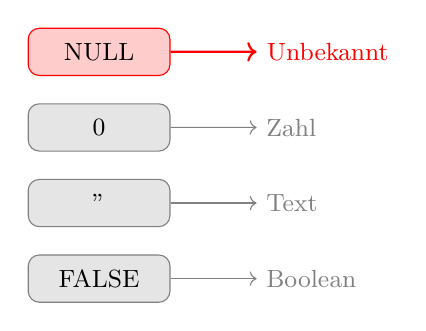
\begin{tikzpicture}[scale=0.8]
    \node[nullbox, fill=red!20, draw=red] (null) at (0,3) {NULL};
    \node[nullbox] (zero) at (0,1.8) {0};
    \node[nullbox] (empty) at (0,0.6) {''};
    \node[nullbox] (false) at (0,-0.6) {FALSE};

    \draw[red, thick, ->] (null) -- ++(2.5,0) node[right, font=\small] {Unbekannt};
    \draw[gray, ->] (zero) -- ++(2.5,0) node[right, font=\small] {Zahl};
    \draw[gray, ->] (empty) -- ++(2.5,0) node[right, font=\small] {Text};
    \draw[gray, ->] (false) -- ++(2.5,0) node[right, font=\small] {Boolean};
\end{tikzpicture}
\end{column}
\end{columns}

\end{frame}

\begin{frame}{Warum NULL wichtig ist}

\textbf{Reales Beispiel:} Spieler-Datenbank

\vspace{0.3cm}

\begin{center}
\small
\begin{tabular}{llrrr}
\toprule
\textbf{Name} & \textbf{Verein} & \textbf{Tore} & \textbf{Vorlagen} & \textbf{Spitzname} \\
\midrule
Müller & Bayern & 8 & 4 & Mülli \\
Neuer & Bayern & 0 & NULL & NULL \\
Gündogan & NULL & NULL & 2 & Günni \\
Musiala & Bayern & 12 & 7 & NULL \\
\bottomrule
\end{tabular}
\end{center}

\vspace{0.3cm}

\begin{itemize}
    \item Neuer: 0 Tore (bekannt!), Vorlagen unbekannt
    \item Gündogan: Verein fehlt (vereinslos?), Tore nicht erfasst
    \item Musiala: Hat keinen bekannten Spitznamen
\end{itemize}

\vspace{0.3cm}

\begin{alertblock}{Problem}
Wie rechnen wir mit NULL? Was ist 5 + NULL? Was ist NULL > 10?
\end{alertblock}

\end{frame}

\begin{frame}[fragile]{NULL prüfen: IS NULL / IS NOT NULL}

\begin{alertblock}{Wichtig}
\texttt{= NULL} funktioniert \textbf{nicht}! Verwende \texttt{IS NULL}.
\end{alertblock}

\vspace{0.3cm}

\begin{columns}[T]
\begin{column}{0.48\textwidth}
\textbf{\textcolor{red}{\ding{55}} Falsch:}
\begin{lstlisting}
SELECT *
FROM spieler
WHERE Tore = NULL;
\end{lstlisting}
{\small\color{red} $\rightarrow$ Liefert \textbf{keine} Ergebnisse!}

\vspace{0.3cm}

\textbf{Warum?}\\
{\small NULL = NULL ist nicht TRUE, sondern UNKNOWN!}
\end{column}

\begin{column}{0.48\textwidth}
\textbf{\textcolor{green!60!black}{\ding{51}} Richtig:}
\begin{lstlisting}
SELECT *
FROM spieler
WHERE Tore IS NULL;
\end{lstlisting}
{\small $\rightarrow$ Alle Spieler ohne Tor-Angabe}

\vspace{0.3cm}

\begin{lstlisting}
SELECT *
FROM spieler
WHERE Tore IS NOT NULL;
\end{lstlisting}
{\small $\rightarrow$ Alle mit Tor-Angabe}
\end{column}
\end{columns}

\end{frame}

\begin{frame}{Dreiwertige Logik}

Mit NULL gibt es \textbf{drei} mögliche Wahrheitswerte:

\vspace{0.3cm}

\begin{center}
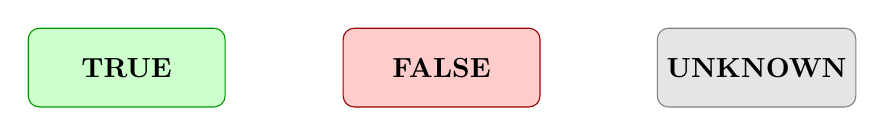
\begin{tikzpicture}
    \node[rectangle, rounded corners, draw=green!60!black, fill=green!20,
          minimum width=2.5cm, minimum height=1cm] (true) at (0,0) {\textbf{TRUE}};
    \node[rectangle, rounded corners, draw=red!60!black, fill=red!20,
          minimum width=2.5cm, minimum height=1cm] (false) at (4,0) {\textbf{FALSE}};
    \node[rectangle, rounded corners, draw=gray, fill=gray!20,
          minimum width=2.5cm, minimum height=1cm] (unknown) at (8,0) {\textbf{UNKNOWN}};
\end{tikzpicture}
\end{center}

\vspace{0.5cm}

\begin{exampleblock}{Beispiele}
\begin{itemize}
    \item \texttt{5 > 3} $\rightarrow$ TRUE
    \item \texttt{5 < 3} $\rightarrow$ FALSE
    \item \texttt{5 > NULL} $\rightarrow$ UNKNOWN (Wir wissen nicht, ob 5 größer ist!)
    \item \texttt{NULL = NULL} $\rightarrow$ UNKNOWN (Nicht TRUE!)
\end{itemize}
\end{exampleblock}

\vspace{0.3cm}

\begin{block}{Konsequenz}
\texttt{WHERE} gibt nur Zeilen zurück, bei denen die Bedingung \textbf{TRUE} ist -- nicht UNKNOWN!
\end{block}

\end{frame}

\begin{frame}{Wahrheitstabellen mit NULL}

\begin{columns}[T]
\begin{column}{0.32\textwidth}
\textbf{AND mit NULL}\\[0.5em]
\small
\begin{tabular}{cc|c}
A & B & A AND B \\
\hline
T & ? & ? \\
F & ? & \textbf{F} \\
? & ? & ? \\
\end{tabular}

\vspace{0.3cm}

{\footnotesize FALSE ``gewinnt'' immer}
\end{column}

\begin{column}{0.32\textwidth}
\textbf{OR mit NULL}\\[0.5em]
\small
\begin{tabular}{cc|c}
A & B & A OR B \\
\hline
T & ? & \textbf{T} \\
F & ? & ? \\
? & ? & ? \\
\end{tabular}

\vspace{0.3cm}

{\footnotesize TRUE ``gewinnt'' immer}
\end{column}

\begin{column}{0.32\textwidth}
\textbf{NOT mit NULL}\\[0.5em]
\small
\begin{tabular}{c|c}
A & NOT A \\
\hline
T & F \\
F & T \\
? & ? \\
\end{tabular}

\vspace{0.3cm}

{\footnotesize Bleibt UNKNOWN}
\end{column}
\end{columns}

\vspace{0.5cm}

\begin{alertblock}{Merkregel}
\texttt{?} = UNKNOWN. Wenn das Ergebnis \textbf{nicht sicher} bestimmt werden kann, bleibt es UNKNOWN.\\
\textbf{Ausnahme:} FALSE AND anything = FALSE, TRUE OR anything = TRUE
\end{alertblock}

\end{frame}

\begin{frame}[fragile]{COALESCE: NULL ersetzen}

\begin{block}{Syntax}
\begin{lstlisting}
COALESCE(wert1, wert2, wert3, ...)
\end{lstlisting}
Gibt den \textbf{ersten Nicht-NULL-Wert} zurück.
\end{block}

\vspace{0.5cm}

\begin{lstlisting}
SELECT
    Name,
    Tore AS Tore_Original,
    COALESCE(Tore, 0) AS Tore_Bereinigt
FROM spieler;
\end{lstlisting}

\vspace{0.3cm}

\begin{center}
\small
\begin{tabular}{lrr}
\toprule
\textbf{Name} & \textbf{Tore\_Original} & \textbf{Tore\_Bereinigt} \\
\midrule
Müller & 8 & 8 \\
Neuer & 0 & 0 \\
Gündogan & NULL & 0 \\
\bottomrule
\end{tabular}
\end{center}

\end{frame}

\begin{frame}[fragile]{COALESCE: Schritt für Schritt}

\textbf{Aufgabe:} Zeige alle Spieler mit Toren, ersetze NULL durch 0.

\vspace{0.3cm}

\begin{enumerate}
    \item \textbf{Was zeigen?} $\rightarrow$ Name und Tore
    \item \textbf{NULL ersetzen?} $\rightarrow$ Ja, mit COALESCE
    \item \textbf{Ersatzwert?} $\rightarrow$ 0
\end{enumerate}

\vspace{0.3cm}

\begin{lstlisting}
SELECT
    Name,
    COALESCE(Tore, 0) AS Tore
FROM spieler;
\end{lstlisting}

\vspace{0.3cm}

\begin{exampleblock}{Wie COALESCE funktioniert}
\texttt{COALESCE(NULL, 0)} $\rightarrow$ 0 (erster Wert ist NULL, also nimm zweiten)\\
\texttt{COALESCE(8, 0)} $\rightarrow$ 8 (erster Wert ist nicht NULL, nimm ihn)\\
\texttt{COALESCE(NULL, NULL, 5)} $\rightarrow$ 5 (erst der dritte ist nicht NULL)
\end{exampleblock}

\end{frame}

\begin{frame}[fragile]{COALESCE: Mehrere Fallbacks}

\begin{lstlisting}
SELECT
    Name,
    COALESCE(Spitzname, Vorname, Name) AS Anzeigename
FROM spieler;
\end{lstlisting}

\vspace{0.5cm}

\textbf{Logik:}
\begin{enumerate}
    \item Wenn Spitzname vorhanden $\rightarrow$ nimm Spitzname
    \item Sonst wenn Vorname vorhanden $\rightarrow$ nimm Vorname
    \item Sonst $\rightarrow$ nimm Name
\end{enumerate}

\vspace{0.3cm}

\begin{center}
\small
\begin{tabular}{llll}
\toprule
\textbf{Name} & \textbf{Spitzname} & \textbf{Vorname} & \textbf{Anzeigename} \\
\midrule
Müller & Mülli & Thomas & Mülli \\
Neuer & NULL & Manuel & Manuel \\
Musiala & NULL & Jamal & Jamal \\
\bottomrule
\end{tabular}
\end{center}

\end{frame}

\begin{frame}[fragile]{Rechnen mit NULL}

\begin{alertblock}{Problem}
Jede Rechnung mit NULL ergibt NULL!
\end{alertblock}

\vspace{0.3cm}

\begin{lstlisting}
-- Problem: Scorerpunkte berechnen
SELECT Name, Tore + Vorlagen AS Scorerpunkte
FROM spieler;
\end{lstlisting}

\begin{center}
\small
\begin{tabular}{lrrl}
Name & Tore & Vorlagen & Scorerpunkte \\
\hline
Müller & 8 & 4 & 12 \\
Neuer & 0 & NULL & \textbf{NULL} \\
Gündogan & NULL & 2 & \textbf{NULL} \\
\end{tabular}
\end{center}

\begin{lstlisting}
-- Lösung: COALESCE verwenden
SELECT Name,
       COALESCE(Tore, 0) + COALESCE(Vorlagen, 0) AS Scorerpunkte
FROM spieler;
\end{lstlisting}

Jetzt: Neuer = 0, Gündogan = 2

\end{frame}

\begin{frame}{NULL: Zusammenfassung}

\begin{center}
\begin{tabular}{ll}
\toprule
\textbf{Situation} & \textbf{Lösung} \\
\midrule
NULL prüfen & \texttt{IS NULL} / \texttt{IS NOT NULL} \\
NULL ersetzen & \texttt{COALESCE(wert, ersatz)} \\
Rechnen mit NULL & Vorher mit COALESCE ersetzen \\
Vergleich mit NULL & \texttt{IS NULL} (nicht \texttt{= NULL}!) \\
\bottomrule
\end{tabular}
\end{center}

\vspace{0.5cm}

\begin{block}{Goldene Regeln}
\begin{enumerate}
    \item NULL ist nicht 0, nicht '', nicht FALSE -- es ist \textbf{unbekannt}
    \item Verwende \texttt{IS NULL}, niemals \texttt{= NULL}
    \item Bei Berechnungen: erst NULL behandeln mit COALESCE
    \item WHERE filtert UNKNOWN als FALSE
\end{enumerate}
\end{block}

\end{frame}

%%%%%%%%%%%%%%%%%%%%%%%%%%%%%%%%%%%%%%%%%%%%%%%%%%%%%%%%%%%%%%%%%%%%%%%%%%%%%%%%%%%%%
% HANDS-ON Phase 6
%%%%%%%%%%%%%%%%%%%%%%%%%%%%%%%%%%%%%%%%%%%%%%%%%%%%%%%%%%%%%%%%%%%%%%%%%%%%%%%%%%%%%

{
\setbeamercolor{background canvas}{bg=IMSOrange!15}
\begin{frame}[plain]
\vfill
\begin{center}
{\Huge\color{IMSOrange} Hands-on}\\[1em]
{\Large Umgang mit NULL}\\[2em]
{\large\ttfamily marimo: 02-sql-exploration.py}\\[1em]
{\normalsize Aufgaben 6.1 -- 6.12}\\[0.5em]
{\small 40 Minuten -- Debugging \& Freie Exploration}
\end{center}
\vfill
\end{frame}
}

%%%%%%%%%%%%%%%%%%%%%%%%%%%%%%%%%%%%%%%%%%%%%%%%%%%%%%%%%%%%%%%%%%%%%%%%%%%%%%%%%%%%%
\section{Visualisierung: Streudiagramme}
%%%%%%%%%%%%%%%%%%%%%%%%%%%%%%%%%%%%%%%%%%%%%%%%%%%%%%%%%%%%%%%%%%%%%%%%%%%%%%%%%%%%%

\showagenda{4}

\begin{frame}[fragile]{Streudiagramm: Zusammenhänge erkennen}

\textbf{Neu:} \texttt{px.scatter()} -- zeigt Beziehung zwischen zwei Variablen

\vspace{0.5cm}

\textbf{Frage:} Wer schießt viele Tore, kassiert aber auch viele?

\begin{lstlisting}
SELECT Mannschaft, ToreGeschossen, ToreKassiert
FROM bundesliga;
\end{lstlisting}

\vspace{0.3cm}

\begin{lstlisting}[language=Python, morekeywords={px}]
px.scatter(ergebnis,
           x="ToreGeschossen",
           y="ToreKassiert",
           hover_name="Mannschaft",
           title="Offensive vs. Defensive")
\end{lstlisting}

\vspace{0.3cm}

$\Rightarrow$ Jeder Punkt = ein Team. Hover zeigt den Namen.

\end{frame}

\begin{frame}{Streudiagramm lesen}

\begin{columns}
\begin{column}{0.5\textwidth}
\textbf{Quadranten:}
\begin{itemize}
    \item \textbf{Oben rechts:} Viele Tore, viele kassiert\\
    {\small (offensiv, aber anfällig)}
    \item \textbf{Unten rechts:} Viele Tore, wenig kassiert\\
    {\small (Spitzenteams)}
    \item \textbf{Unten links:} Wenig Tore, wenig kassiert\\
    {\small (defensiv, langweilig)}
    \item \textbf{Oben links:} Wenig Tore, viele kassiert\\
    {\small (Abstiegskandidaten)}
\end{itemize}
\end{column}

\begin{column}{0.5\textwidth}
\begin{tikzpicture}[scale=0.8]
    \draw[->] (0,0) -- (5,0) node[right, font=\small] {Tore};
    \draw[->] (0,0) -- (0,4) node[above, font=\small] {Kassiert};
    \draw[dashed, gray] (2.5,0) -- (2.5,4);
    \draw[dashed, gray] (0,2) -- (5,2);
    \node[font=\tiny, text=red] at (1.2,3) {Abstieg};
    \node[font=\tiny, text=gray] at (1.2,1) {Defensiv};
    \node[font=\tiny, text=IMSOrange] at (3.8,3) {Spektakel};
    \node[font=\tiny, text=green!60!black] at (3.8,1) {Top};
\end{tikzpicture}
\end{column}
\end{columns}

\end{frame}

\begin{frame}[fragile]{Farbe für Kategorien}

\textbf{Neu:} \texttt{color=} -- färbt Punkte nach einer Kategorie

\vspace{0.5cm}

\begin{lstlisting}[language=Python, morekeywords={px}]
px.scatter(ergebnis,
           x="ToreGeschossen",
           y="ToreKassiert",
           color="Liga",  -- kategoriale Variable!
           hover_name="Mannschaft")
\end{lstlisting}

\vspace{0.5cm}

\textbf{Wann \texttt{color=} verwenden?}
\begin{itemize}
    \item Gruppen vergleichen (Liga, Position, Kategorie)
    \item Muster zwischen Gruppen erkennen
    \item \textbf{Nicht:} für kontinuierliche Werte wie Punkte
\end{itemize}

\end{frame}

%%%%%%%%%%%%%%%%%%%%%%%%%%%%%%%%%%%%%%%%%%%%%%%%%%%%%%%%%%%%%%%%%%%%%%%%%%%%%%%%%%%%%
\section{Zusammenfassung}
%%%%%%%%%%%%%%%%%%%%%%%%%%%%%%%%%%%%%%%%%%%%%%%%%%%%%%%%%%%%%%%%%%%%%%%%%%%%%%%%%%%%%

\showagenda{5}

\begin{frame}{SQL-Ausführungsreihenfolge (komplett)}

\begin{center}
\begin{tikzpicture}[node distance=0.4cm]
    \node[sqlbox, minimum width=3.5cm] (from) {1. FROM};
    \node[sqlbox, minimum width=3.5cm, below=of from] (where) {2. WHERE};
    \node[sqlbox, minimum width=3.5cm, below=of where] (select) {3. SELECT};
    \node[sqlbox, minimum width=3.5cm, below=of select] (distinct) {4. DISTINCT};
    \node[sqlbox, minimum width=3.5cm, below=of distinct] (order) {5. ORDER BY};
    \node[sqlbox, minimum width=3.5cm, below=of order, fill=IMSOrange!20, draw=IMSOrange] (limit) {6. LIMIT};

    \draw[sqlarrow] (from) -- (where);
    \draw[sqlarrow] (where) -- (select);
    \draw[sqlarrow] (select) -- (distinct);
    \draw[sqlarrow] (distinct) -- (order);
    \draw[sqlarrow] (order) -- (limit);

    \node[right=0.5cm of from, font=\small\color{gray}] {Tabelle laden};
    \node[right=0.5cm of where, font=\small\color{gray}] {Zeilen filtern};
    \node[right=0.5cm of select, font=\small\color{gray}] {Spalten wählen};
    \node[right=0.5cm of distinct, font=\small\color{gray}] {Duplikate entfernen};
    \node[right=0.5cm of order, font=\small\color{gray}] {Sortieren};
    \node[right=0.5cm of limit, font=\small\color{gray}] {Begrenzen};
\end{tikzpicture}
\end{center}

\end{frame}

\begin{frame}[fragile]{Was wir heute gelernt haben}

\begin{columns}
\begin{column}{0.5\textwidth}
\begin{tabular}{ll}
\toprule
\textbf{SQL} & \textbf{Syntax} \\
\midrule
Aufsteigend & \texttt{ORDER BY x ASC} \\
Absteigend & \texttt{ORDER BY x DESC} \\
Begrenzen & \texttt{LIMIT n} \\
Überspringen & \texttt{OFFSET m} \\
Eindeutig & \texttt{DISTINCT} \\
NULL prüfen & \texttt{IS NULL} \\
NULL ersetzen & \texttt{COALESCE()} \\
\bottomrule
\end{tabular}
\end{column}

\begin{column}{0.5\textwidth}
\begin{tabular}{ll}
\toprule
\textbf{Visualisierung} & \textbf{Funktion} \\
\midrule
Balkendiagramm & \texttt{px.bar()} \\
Streudiagramm & \texttt{px.scatter()} \\
Histogramm & \texttt{px.histogram()} \\
Liniendiagramm & \texttt{px.line()} \\
Kreisdiagramm & \texttt{px.pie()} \\
\bottomrule
\end{tabular}
\end{column}
\end{columns}

\vspace{0.3cm}

\begin{block}{Workflow}
SQL-Abfrage $\rightarrow$ DataFrame $\rightarrow$ Plotly Chart
\end{block}

\end{frame}

\begin{frame}{Quiz 1: ORDER BY}

\textbf{Was zeigt diese Abfrage?}

\vspace{0.3cm}

\texttt{SELECT Mannschaft, Punkte FROM bundesliga ORDER BY Punkte LIMIT 3;}

\vspace{0.5cm}

\begin{enumerate}
    \item Die 3 Teams mit den meisten Punkten
    \item Die 3 Teams mit den wenigsten Punkten
    \item Die ersten 3 Teams alphabetisch
    \item Einen Fehler
\end{enumerate}

\end{frame}

\begin{frame}{Quiz 1: Lösung}

\textbf{Was zeigt diese Abfrage?}

\vspace{0.3cm}

\texttt{SELECT Mannschaft, Punkte FROM bundesliga ORDER BY Punkte LIMIT 3;}

\vspace{0.5cm}

\begin{enumerate}
    \item Die 3 Teams mit den meisten Punkten
    \item \textbf{\textcolor{green!60!black}{Die 3 Teams mit den wenigsten Punkten}}
    \item Die ersten 3 Teams alphabetisch
    \item Einen Fehler
\end{enumerate}

\vspace{0.5cm}

\begin{block}{Erklärung}
\texttt{ORDER BY Punkte} ohne ASC/DESC sortiert \textbf{aufsteigend} (ASC ist Default).\\
Also: kleinste Werte zuerst $\rightarrow$ Abstiegskandidaten!
\end{block}

\end{frame}

\begin{frame}{Quiz 2: NULL}

\textbf{Was ist das Ergebnis von:}

\vspace{0.3cm}

\texttt{SELECT * FROM spieler WHERE Tore > 5 OR Tore <= 5;}

\vspace{0.5cm}

\begin{enumerate}
    \item Alle Spieler
    \item Nur Spieler mit Tore-Wert (nicht NULL)
    \item Nur Spieler mit mehr als 5 Toren
    \item Leeres Ergebnis
\end{enumerate}

\end{frame}

\begin{frame}{Quiz 2: Lösung}

\textbf{Was ist das Ergebnis von:}

\vspace{0.3cm}

\texttt{SELECT * FROM spieler WHERE Tore > 5 OR Tore <= 5;}

\vspace{0.5cm}

\begin{enumerate}
    \item Alle Spieler
    \item \textbf{\textcolor{green!60!black}{Nur Spieler mit Tore-Wert (nicht NULL)}}
    \item Nur Spieler mit mehr als 5 Toren
    \item Leeres Ergebnis
\end{enumerate}

\vspace{0.5cm}

\begin{block}{Erklärung}
Wenn Tore NULL ist:\\
\texttt{NULL > 5} $\rightarrow$ UNKNOWN\\
\texttt{NULL <= 5} $\rightarrow$ UNKNOWN\\
\texttt{UNKNOWN OR UNKNOWN} $\rightarrow$ UNKNOWN\\
WHERE filtert UNKNOWN als FALSE $\rightarrow$ Zeile wird nicht angezeigt!
\end{block}

\end{frame}

\begin{frame}{Quiz 3: COALESCE}

\textbf{Was gibt \texttt{COALESCE(NULL, NULL, 'Hallo', 'Welt')} zurück?}

\vspace{0.5cm}

\begin{enumerate}
    \item NULL
    \item 'Hallo'
    \item 'Welt'
    \item 'Hallo Welt'
\end{enumerate}

\end{frame}

\begin{frame}{Quiz 3: Lösung}

\textbf{Was gibt \texttt{COALESCE(NULL, NULL, 'Hallo', 'Welt')} zurück?}

\vspace{0.5cm}

\begin{enumerate}
    \item NULL
    \item \textbf{\textcolor{green!60!black}{'Hallo'}}
    \item 'Welt'
    \item 'Hallo Welt'
\end{enumerate}

\vspace{0.5cm}

\begin{block}{Erklärung}
COALESCE gibt den \textbf{ersten Nicht-NULL-Wert} zurück:
\begin{itemize}
    \item Argument 1: NULL $\rightarrow$ weiter
    \item Argument 2: NULL $\rightarrow$ weiter
    \item Argument 3: 'Hallo' $\rightarrow$ \textbf{gefunden!}
\end{itemize}
'Welt' wird gar nicht mehr betrachtet.
\end{block}

\end{frame}

\begin{frame}{Cheat Sheet: Vorlesung 2}

\begin{center}
\small
\begin{tabular}{ll}
\toprule
\textbf{Konzept} & \textbf{Syntax} \\
\midrule
Aufsteigend sortieren & \texttt{ORDER BY spalte ASC} \\
Absteigend sortieren & \texttt{ORDER BY spalte DESC} \\
Top N & \texttt{ORDER BY spalte DESC LIMIT N} \\
Bottom N & \texttt{ORDER BY spalte ASC LIMIT N} \\
Plätze X bis Y & \texttt{LIMIT (Y-X+1) OFFSET (X-1)} \\
\midrule
Eindeutige Werte & \texttt{SELECT DISTINCT spalte} \\
Muster (beginnt mit) & \texttt{LIKE 'Text\%'} \\
Muster (enthält) & \texttt{LIKE '\%Text\%'} \\
Muster (endet mit) & \texttt{LIKE '\%Text'} \\
\midrule
NULL finden & \texttt{WHERE spalte IS NULL} \\
Nicht NULL & \texttt{WHERE spalte IS NOT NULL} \\
NULL ersetzen & \texttt{COALESCE(spalte, ersatz)} \\
\bottomrule
\end{tabular}
\end{center}

\end{frame}

\begin{frame}{Ausblick: Vorlesung 3}

\textbf{Vorlesung 3: Aggregation \& Gruppierung}

\begin{itemize}
    \item Aggregatfunktionen: \texttt{COUNT}, \texttt{SUM}, \texttt{AVG}, \texttt{MIN}, \texttt{MAX}
    \item Gruppierung mit \texttt{GROUP BY}
    \item Filter auf Gruppen mit \texttt{HAVING}
    \item Unterschied \texttt{WHERE} vs. \texttt{HAVING}
\end{itemize}

\vspace{0.5cm}

\begin{exampleblock}{Vorgeschmack}
\begin{itemize}
    \item Wie viele Teams haben mehr als 10 Siege? $\rightarrow$ COUNT
    \item Was ist der Punktedurchschnitt? $\rightarrow$ AVG
    \item Wie viele Tore wurden insgesamt geschossen? $\rightarrow$ SUM
    \item Welches Team hat die meisten Tore? $\rightarrow$ MAX
\end{itemize}
\end{exampleblock}

\end{frame}

\begin{frame}{}
\vfill
\begin{center}
{\Huge Fragen?}

\vspace{1.5em}

{\large\ttfamily marimo: 02-sql-exploration.py}

\vspace{0.5em}

{\small Weiter experimentieren!}
\end{center}
\vfill
\end{frame}

\end{document}
